\documentclass[
    fontsize=12pt,          % default font size 12pt
    paper=a4,               % DIN A4 page format
    numbers=noenddot,       % remove dots behind chapter numbers (e.g. 1.5 not 1.5.)
    listof=totoc,           % add list of figures, tables, etc. to ToC
    listof=entryprefix,     % add entry name to figures, tables, etc.
    listof=nochaptergap,    % no chapter gap for figures, tables, etc.
    bibliography=totoc,     % add bibliography to ToC but without a chapter number
    parskip=half,           % half line spacing between paragraphs
    openany                 % chapters can start on any page
]{scrbook}

\include{../../for_latex/preamble}

\usepackage{pgfplots}
\pgfplotsset{compat=1.18}
\usepgfplotslibrary{statistics}
\usepackage{pgfplotstable}
\usepackage{amssymb}

\begin{document}

    \begin{titlepage}
        \pagestyle{empty}

        % HFU Logo
        \begin{flushright}
            \begin{figure}[ht]
                \flushright
                
\includegraphics[height=2cm]{../../for_latex/hfu}
            \end{figure}
        \end{flushright}

        \begin{center}
            \vspace{3cm}

            {\fontsize{22}{22} \selectfont \textbf{Blatt 3}}\\[5mm]
            {\fontsize{18}{18} \selectfont Kryptologie}

            \vspace{12cm}

            {\fontsize{14}{14} \selectfont Luis Staudt}
        \end{center}
    \end{titlepage}

% ############################################################################
% CONTENT STARTS HERE
% ############################################################################


\chapter*{Konfusion und Diffusion beim Present}


\section*{Aufgabenstellung}

Es soll der Lightweight-Block-Cipher Present (ISO/IEC 29192-2) hinsichtlich Konfusion und Diffusion analysiert werden.
Dazu wird der 64-Bit-ALL-ZERO Plaintext sowie alle 64 Plaintexte mit Hamming-Gewicht~1 mit einem 128-Bit-Schlüssel verschlüsselt, der aus dem zyklisch fortgesetzten Vornamen \texttt{Luis} in ASCII besteht.

Für jede der 31~Runden werden untersucht:
\begin{itemize}
    \item \textbf{Diffusion:} Hamming-Abstände zwischen den Rundenstates des ALL-ZERO Plaintexts und der Hamming-Weight-1 Plaintexte
    \item \textbf{Konfusion:} Häufigkeitsverteilung der Nibble-Werte über alle $65 \cdot 16 = 1040$ State-Nibbles pro Runde
\end{itemize}


\section*{Vorgehensweise}

Die Implementierung erfolgt in Java.
Der Present-Cipher wird mit 128-Bit-Schlüssel gemäß der Spezifikation implementiert: 31~Runden mit S-Box-Substitution, Bit-Permutation (P-Layer) und Rundenschlüssel-Addition, gefolgt von einer finalen Schlüssel-Addition.

Der Schlüssel ergibt sich aus \texttt{Luis} zyklisch fortgesetzt auf 16~Bytes:
\[
    \text{Key} = \texttt{0x4C7569734C7569734C7569734C756973}
\]

\begin{lstlisting}[language=Java, caption={Present-Rundenfunktion}]
static long presentEncrypt(long plaintext, long[] roundKeys, long[] states) {
    long state = plaintext;
    for (int i = 0; i < 31; i++) {
        state ^= roundKeys[i];
        state = sBoxLayer(state);
        state = pLayer(state);
        if (states != null) states[i] = state;
    }
    return state ^ roundKeys[31];
}
\end{lstlisting}

Die Korrektheit wird mit dem Testvektor aus der Spezifikation verifiziert:
\begin{itemize}
    \item Key = \texttt{0x00...00}, Plaintext = \texttt{0x00...00} $\rightarrow$ Ciphertext = \texttt{0x96DB702A2E6900AF} \checkmark
\end{itemize}


\section*{Ergebnisse}


\subsection*{Ciphertexte}

\begin{table}[H]
    \centering
    \begin{tabular}{l l}
        \toprule
        \textbf{Plaintext} & \textbf{Ciphertext} \\
        \midrule
        ALL-ZERO (\texttt{0x0000000000000000}) & \texttt{0xA306783D564F96E0} \\
        Bit 0 (\texttt{0x0000000000000001})    & \texttt{0xDCCDF938AE3EB7B4} \\
        Bit 15 (\texttt{0x0000000000008000})   & \texttt{0x6EE65CE221F3FF71} \\
        Bit 31 (\texttt{0x0000000080000000})   & \texttt{0xCBAE2361D1FCEF6C} \\
        Bit 47 (\texttt{0x0000800000000000})   & \texttt{0xFC3784BF0E853779} \\
        Bit 63 (\texttt{0x8000000000000000})   & \texttt{0xD279D888ADDEC85E} \\
        \bottomrule
    \end{tabular}
    \caption{Ausgewählte Ciphertexte}
\end{table}


\subsection*{Diffusion -- Hamming-Abstände}

Für jede Runde werden die Hamming-Abstände zwischen dem Rundenstate des ALL-ZERO Plaintexts und den Rundenstates der 64~Hamming-Weight-1 Plaintexte berechnet.
Bei idealer Diffusion erwartet man einen mittleren Hamming-Abstand von 32 (die Hälfte der 64~State-Bits).

\begin{figure}[H]
    \centering
    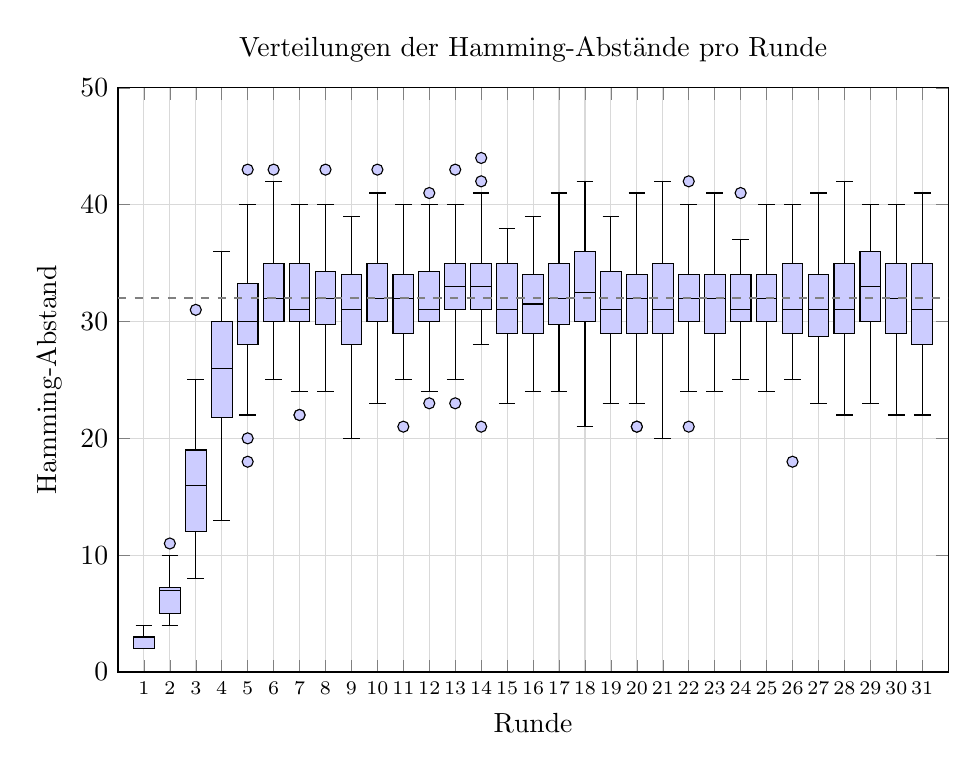
\begin{tikzpicture}
        \begin{axis}[
            boxplot/draw direction=y,
            width=\textwidth,
            height=9cm,
            xlabel={Runde},
            ylabel={Hamming-Abstand},
            title={Verteilungen der Hamming-Abstände pro Runde},
            xtick={1,2,...,31},
            x tick label style={font=\scriptsize},
            xmin=0, xmax=32,
            ymin=0, ymax=50,
            grid=major,
            grid style={gray!30},
        ]
        \addplot[boxplot prepared={draw position=1, lower whisker=2, lower quartile=2.00, median=3.00, upper quartile=3.00, upper whisker=4}, fill=blue!20] coordinates {};
\addplot[boxplot prepared={draw position=2, lower whisker=4, lower quartile=5.00, median=7.00, upper quartile=7.25, upper whisker=10}, fill=blue!20] coordinates { (0,11) };
\addplot[boxplot prepared={draw position=3, lower whisker=8, lower quartile=12.00, median=16.00, upper quartile=19.00, upper whisker=25}, fill=blue!20] coordinates { (0,31) };
\addplot[boxplot prepared={draw position=4, lower whisker=13, lower quartile=21.75, median=26.00, upper quartile=30.00, upper whisker=36}, fill=blue!20] coordinates {};
\addplot[boxplot prepared={draw position=5, lower whisker=22, lower quartile=28.00, median=30.00, upper quartile=33.25, upper whisker=40}, fill=blue!20] coordinates { (0,18) (0,20) (0,43) };
\addplot[boxplot prepared={draw position=6, lower whisker=25, lower quartile=30.00, median=32.00, upper quartile=35.00, upper whisker=42}, fill=blue!20] coordinates { (0,43) };
\addplot[boxplot prepared={draw position=7, lower whisker=24, lower quartile=30.00, median=31.00, upper quartile=35.00, upper whisker=40}, fill=blue!20] coordinates { (0,22) (0,22) };
\addplot[boxplot prepared={draw position=8, lower whisker=24, lower quartile=29.75, median=32.00, upper quartile=34.25, upper whisker=40}, fill=blue!20] coordinates { (0,43) };
\addplot[boxplot prepared={draw position=9, lower whisker=20, lower quartile=28.00, median=31.00, upper quartile=34.00, upper whisker=39}, fill=blue!20] coordinates {};
\addplot[boxplot prepared={draw position=10, lower whisker=23, lower quartile=30.00, median=32.00, upper quartile=35.00, upper whisker=41}, fill=blue!20] coordinates { (0,43) };
\addplot[boxplot prepared={draw position=11, lower whisker=25, lower quartile=29.00, median=32.00, upper quartile=34.00, upper whisker=40}, fill=blue!20] coordinates { (0,21) };
\addplot[boxplot prepared={draw position=12, lower whisker=24, lower quartile=30.00, median=31.00, upper quartile=34.25, upper whisker=40}, fill=blue!20] coordinates { (0,23) (0,41) };
\addplot[boxplot prepared={draw position=13, lower whisker=25, lower quartile=31.00, median=33.00, upper quartile=35.00, upper whisker=40}, fill=blue!20] coordinates { (0,23) (0,43) };
\addplot[boxplot prepared={draw position=14, lower whisker=28, lower quartile=31.00, median=33.00, upper quartile=35.00, upper whisker=41}, fill=blue!20] coordinates { (0,21) (0,42) (0,44) };
\addplot[boxplot prepared={draw position=15, lower whisker=23, lower quartile=29.00, median=31.00, upper quartile=35.00, upper whisker=38}, fill=blue!20] coordinates {};
\addplot[boxplot prepared={draw position=16, lower whisker=24, lower quartile=29.00, median=31.50, upper quartile=34.00, upper whisker=39}, fill=blue!20] coordinates {};
\addplot[boxplot prepared={draw position=17, lower whisker=24, lower quartile=29.75, median=32.00, upper quartile=35.00, upper whisker=41}, fill=blue!20] coordinates {};
\addplot[boxplot prepared={draw position=18, lower whisker=21, lower quartile=30.00, median=32.50, upper quartile=36.00, upper whisker=42}, fill=blue!20] coordinates {};
\addplot[boxplot prepared={draw position=19, lower whisker=23, lower quartile=29.00, median=31.00, upper quartile=34.25, upper whisker=39}, fill=blue!20] coordinates {};
\addplot[boxplot prepared={draw position=20, lower whisker=23, lower quartile=29.00, median=32.00, upper quartile=34.00, upper whisker=41}, fill=blue!20] coordinates { (0,21) (0,21) };
\addplot[boxplot prepared={draw position=21, lower whisker=20, lower quartile=29.00, median=31.00, upper quartile=35.00, upper whisker=42}, fill=blue!20] coordinates {};
\addplot[boxplot prepared={draw position=22, lower whisker=24, lower quartile=30.00, median=32.00, upper quartile=34.00, upper whisker=40}, fill=blue!20] coordinates { (0,21) (0,42) };
\addplot[boxplot prepared={draw position=23, lower whisker=24, lower quartile=29.00, median=32.00, upper quartile=34.00, upper whisker=41}, fill=blue!20] coordinates {};
\addplot[boxplot prepared={draw position=24, lower whisker=25, lower quartile=30.00, median=31.00, upper quartile=34.00, upper whisker=37}, fill=blue!20] coordinates { (0,41) };
\addplot[boxplot prepared={draw position=25, lower whisker=24, lower quartile=30.00, median=32.00, upper quartile=34.00, upper whisker=40}, fill=blue!20] coordinates {};
\addplot[boxplot prepared={draw position=26, lower whisker=25, lower quartile=29.00, median=31.00, upper quartile=35.00, upper whisker=40}, fill=blue!20] coordinates { (0,18) };
\addplot[boxplot prepared={draw position=27, lower whisker=23, lower quartile=28.75, median=31.00, upper quartile=34.00, upper whisker=41}, fill=blue!20] coordinates {};
\addplot[boxplot prepared={draw position=28, lower whisker=22, lower quartile=29.00, median=31.00, upper quartile=35.00, upper whisker=42}, fill=blue!20] coordinates {};
\addplot[boxplot prepared={draw position=29, lower whisker=23, lower quartile=30.00, median=33.00, upper quartile=36.00, upper whisker=40}, fill=blue!20] coordinates {};
\addplot[boxplot prepared={draw position=30, lower whisker=22, lower quartile=29.00, median=32.00, upper quartile=35.00, upper whisker=40}, fill=blue!20] coordinates {};
\addplot[boxplot prepared={draw position=31, lower whisker=22, lower quartile=28.00, median=31.00, upper quartile=35.00, upper whisker=41}, fill=blue!20] coordinates {};

        \draw[dashed, gray, thick] (axis cs:0,32) -- (axis cs:32,32);
        \end{axis}
    \end{tikzpicture}
    \caption{Boxplot der Hamming-Abstände (gestrichelt: Idealwert 32)}
    \label{fig:hamming}
\end{figure}

\begin{table}[H]
    \centering
    \begin{tabular}{c r r r r}
        \toprule
        \textbf{Runde} & \textbf{Min} & \textbf{Max} & \textbf{Mean} & \textbf{Median} \\
        \midrule
        1  & 2  & 4  & 2{,}6  & 3{,}0 \\
        2  & 4  & 11 & 6{,}5  & 7{,}0 \\
        3  & 8  & 31 & 16{,}0 & 16{,}0 \\
        4  & 13 & 36 & 25{,}6 & 26{,}0 \\
        5  & 18 & 43 & 30{,}4 & 30{,}0 \\
        6  & 25 & 43 & 32{,}2 & 32{,}0 \\
        \midrule
        31 & 22 & 41 & 31{,}3 & 31{,}0 \\
        \bottomrule
    \end{tabular}
    \caption{Hamming-Abstände in ausgewählten Runden}
\end{table}

\textbf{Beobachtungen:}
\begin{itemize}
    \item \textbf{Runde 1--2:} Der Hamming-Abstand ist sehr gering (2--11).
    Ein einzelnes geflipptes Bit beeinflusst nur wenige State-Bits, da die S-Box nur das betroffene Nibble ändert und die P-Schicht die Bits lediglich umordnet.
    \item \textbf{Runde 3--5:} Schneller Anstieg der Hamming-Abstände (Mittelwert von 16 auf 30).
    Der Lawineneffekt setzt ein: Die Kombination aus S-Box (nichtlineare Substitution) und P-Layer (Verteilung der Bits auf verschiedene Nibbles) bewirkt eine exponentielle Ausbreitung der Änderungen.
    \item \textbf{Ab Runde 6:} Die Hamming-Abstände stabilisieren sich um den Idealwert~32 mit einer Streuung von ca.\ $\pm10$.
    Jedes geflippte Eingabebit beeinflusst im Mittel die Hälfte aller State-Bits -- vollständige Diffusion ist erreicht.
\end{itemize}


\subsection*{Konfusion -- Nibble-Verteilungen}

In jeder Runde werden die Nibble-Werte (0--F) über alle 65~States gezählt.
Bei $65 \cdot 16 = 1040$ Nibbles pro Runde beträgt der Erwartungswert bei Gleichverteilung $1040 / 16 = 65$.
Als Maß für die Abweichung von der Gleichverteilung dient die $\chi^2$-Statistik.

\begin{figure}[H]
    \centering
    \begin{tikzpicture}
        \begin{axis}[
            ybar, bar width=8pt,
            width=0.85\textwidth, height=6cm,
            xlabel={Nibble},
            ylabel={Häufigkeit},
            title={Nibble-Verteilung in Runde 1 ($\chi^2 = 1226$)},
            xtick=data,
            xticklabels={0,1,2,3,4,5,6,7,8,9,a,b,c,d,e,f},
            ymin=0,
            grid=major, grid style={gray!30},
            nodes near coords,
            nodes near coords style={font=\tiny, above},
            every node near coord/.append style={rotate=90, anchor=west},
        ]
        \addplot[fill=blue!50] table[x=nibble, y=r1, col sep=comma] {nibble_freq.csv};
        \draw[dashed, red, thick] (axis cs:-0.5,65) -- (axis cs:15.5,65);
        \end{axis}
    \end{tikzpicture}
    \caption{Nibble-Verteilung in Runde 1 -- stark ungleichmäßig}
    \label{fig:nibble1}
\end{figure}

\begin{figure}[H]
    \centering
    \begin{tikzpicture}
        \begin{axis}[
            ybar, bar width=8pt,
            width=0.85\textwidth, height=6cm,
            xlabel={Nibble},
            ylabel={Häufigkeit},
            title={Nibble-Verteilung in Runde 2 ($\chi^2 = 208$)},
            xtick=data,
            xticklabels={0,1,2,3,4,5,6,7,8,9,a,b,c,d,e,f},
            ymin=0,
            grid=major, grid style={gray!30},
            nodes near coords,
            nodes near coords style={font=\tiny, above},
            every node near coord/.append style={rotate=90, anchor=west},
        ]
        \addplot[fill=blue!50] table[x=nibble, y=r2, col sep=comma] {nibble_freq.csv};
        \draw[dashed, red, thick] (axis cs:-0.5,65) -- (axis cs:15.5,65);
        \end{axis}
    \end{tikzpicture}
    \caption{Nibble-Verteilung in Runde 2 -- deutliche Verbesserung}
    \label{fig:nibble2}
\end{figure}

\begin{figure}[H]
    \centering
    \begin{tikzpicture}
        \begin{axis}[
            ybar, bar width=8pt,
            width=0.85\textwidth, height=6cm,
            xlabel={Nibble},
            ylabel={Häufigkeit},
            title={Nibble-Verteilung in Runde 31 ($\chi^2 = 13{,}2$)},
            xtick=data,
            xticklabels={0,1,2,3,4,5,6,7,8,9,a,b,c,d,e,f},
            ymin=0,
            grid=major, grid style={gray!30},
            nodes near coords,
            nodes near coords style={font=\tiny, above},
            every node near coord/.append style={rotate=90, anchor=west},
        ]
        \addplot[fill=blue!50] table[x=nibble, y=r31, col sep=comma] {nibble_freq.csv};
        \draw[dashed, red, thick] (axis cs:-0.5,65) -- (axis cs:15.5,65);
        \end{axis}
    \end{tikzpicture}
    \caption{Nibble-Verteilung in Runde 31 -- annähernde Gleichverteilung}
    \label{fig:nibble31}
\end{figure}

\begin{table}[H]
    \centering
    \begin{tabular}{c r l}
        \toprule
        \textbf{Runde} & $\boldsymbol{\chi^2}$ & \textbf{Beurteilung} \\
        \midrule
        1  & 1226{,}2 & stark ungleichmäßig \\
        2  & 207{,}9  & deutliche Abweichung \\
        3  & 110{,}7  & mäßige Abweichung \\
        4  & 38{,}0   & leichte Abweichung \\
        5  & 22{,}4   & nahe Gleichverteilung \\
        6  & 8{,}1    & annähernd gleichverteilt \\
        \midrule
        31 & 13{,}2   & gleichverteilt \\
        \bottomrule
    \end{tabular}
    \caption{$\chi^2$-Werte der Nibble-Verteilung (Erwartungswert je Nibble: 65)}
\end{table}

\textbf{Beobachtungen:}
\begin{itemize}
    \item \textbf{Runde 1:} Extreme Ungleichverteilung ($\chi^2 = 1226$).
    Die Nibble-Werte 6 und A dominieren mit jeweils über 200~Vorkommen, während andere Werte unter 10 liegen.
    Dies liegt daran, dass die S-Box den Wert 0 auf 0xC abbildet und die meisten Eingabe-Nibbles den Wert~0 haben.
    \item \textbf{Runde 2--4:} Rapide Abnahme des $\chi^2$-Werts.
    Die iterierte Anwendung von S-Box und P-Layer mischt die Nibble-Werte zunehmend.
    \item \textbf{Ab Runde 5--6:} $\chi^2$-Werte schwanken um 10--25, was einer annähernden Gleichverteilung entspricht.
    Der kritische Wert der $\chi^2$-Verteilung mit 15~Freiheitsgraden bei $\alpha = 0{,}05$ beträgt 25{,}0.
    Die meisten Runden ab Runde~6 liegen unterhalb dieses Schwellenwerts.
\end{itemize}


\section*{Bewertung}

Die Analyse zeigt, dass Present innerhalb weniger Runden sowohl vollständige Diffusion als auch gute Konfusion erreicht:

\begin{itemize}
    \item \textbf{Diffusion:} Ab Runde~5--6 beeinflusst ein einzelnes geflipptes Eingabebit im Mittel 32 der 64~State-Bits.
    Der Lawineneffekt wird durch das Zusammenspiel der nichtlinearen S-Box (Konfusion innerhalb eines Nibbles) und des P-Layers (Verteilung der Bits auf verschiedene Nibbles) erzielt.

    \item \textbf{Konfusion:} Ab Runde~5--6 liegt eine annähernde Gleichverteilung der Nibble-Werte vor ($\chi^2 < 25$).
    Die S-Box sorgt für die nichtlineare Vermischung, während der P-Layer die betroffenen Bits über den gesamten State verteilt.

    \item \textbf{Rundenzahl:} Die 31~Runden von Present bieten eine große Sicherheitsmarge.
    Bereits nach 5--6~Runden ist das Diffusions- und Konfusions-Kriterium im Wesentlichen erfüllt.
    Die verbleibenden 25~Runden gewährleisten die kryptographische Sicherheit gegen fortgeschrittene Angriffe wie differenzielle und lineare Kryptoanalyse.
\end{itemize}

% ############################################################################
% CONTENT ENDS HERE
% ############################################################################

\end{document}
